\SACCMD{taper}
\label{cmd:taper}

\SACTitle{概要}
对数据两端应用对称的taper函数,使得数据两端平滑地衰减到零

\SACTitle{语法}
\begin{SACSTX}
TAPER [T!YPE! HAN!NING!|HAM!MING!|C!OSINE!] [W!IDTH! v]
\end{SACSTX}

\SACTitle{输入}
\begin{description}
\item [TYPE HANNING|HAMMIN|COSINE] 应用Hanning、Hamming、余弦衰减窗
\item [WIDTH v] 设置衰减窗的宽度占数据点数的比值为v,v取值在0.0和0.5之间
\end{description}

\SACTitle{缺省值}
\begin{SACDFT}
taper type hanning width 0.05
\end{SACDFT}

\SACTitle{说明}
taper函数是在0和1之间取值的单调函数,若将其对称地施加于数据的首尾两端,
则可实现数据的``尖灭''。

taper函数共计$npts*v$个点,第一个点值为0,最后一个点的值为1,将此函数的
每个点依次于数据的第1至$npts*v$个点相乘,使得数据数据的首端从0开始光滑地
增加到其原始值。数据的末端完全类似,此时数据由其原始值不断光滑地减小到0。

taper命令的通用形式为
\[
    Data(j) = Data(j)*(F_0 - F_1\cos(\omega(j-1)))
\]
此公式应用于数据的首端,另一个完全对称的数据用于数据的尾端。

表 \ref{table:taper-functions} 定义了不同的衰减函数的参数,其中N为
衰减窗的宽度,即$npts*v$。
\begin{table}[ht]
\centering
\caption{taper衰减函数参数一览}
\label{table:taper-functions}
\begin{tabular}{llll}
\toprule
类型 & $\omega$ & $F_0$ & $F_1$ \\
\midrule
HANNING &   $\frac{\pi}{N}$     &   0.50    &   0.50    \\
HAMMING &   $\frac{\pi}{N}$     &   0.54    &   0.46    \\
COSINE  &   $\frac{\pi}{2N}$    &   1.00    &   1.00    \\
\bottomrule
\end{tabular}
\end{table}

图 \ref{fig:taper-functions} 给出了不同taper衰减函数的曲线图,图中可以
看出,hamming窗实际上并没有完全实现尖灭。
\begin{figure}[!ht]
\centering
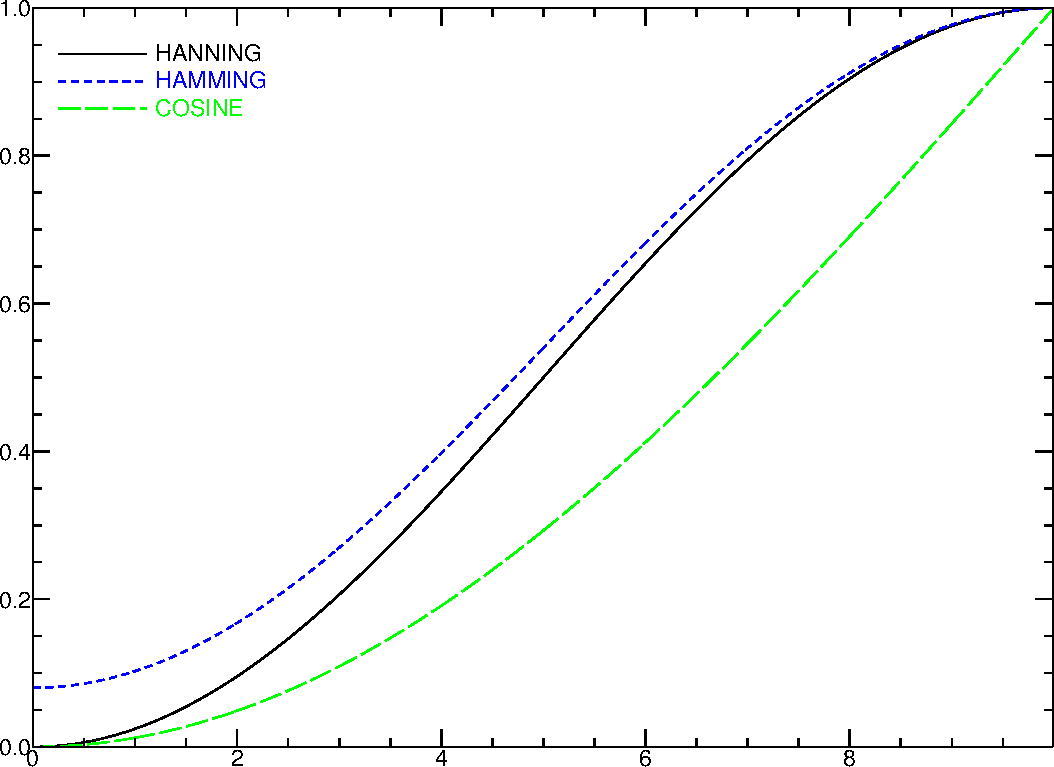
\includegraphics[width=0.8\textwidth]{taper-functions}
\caption{taper衰减函数曲线}
\label{fig:taper-functions}
\end{figure}

\SACTitle{头段变量}
depmin、depmax、depmen
